\subsection{Monotonic-writes consistency}\label{mw:monotonic-writes-consistency}

\subsubsection{Definition}\label{mw:definition}

Monotonic-writes (MW) consistency guarantees that writes issued by the same client are applied in the order the client issued them. For example, suppose a client first writes \(x=1\) and then updates it to \(x=2\). A replica applying both writes should apply the first before the second, even if the requests pass through different coordinators. If it applies them in the reverse order, the earlier write may overwrite the later update, violating MW consistency.

\subsubsection{Experimental Design}\label{mw:experimental-design}

Monotonic writes concern preservation of a client's write order. This experiment examines a specific observable consequence: after sequential overwrites W1 and W2 of the same key, does the reconciled value reflect the later operation W2?

For each iteration, the client writes value 1 through node 2 and waits for completion, then writes value 2 through node 3. Both writes use the selected write consistency level. Verification is performed through node 1 using verify\_cl=ALL in the normal topology. The query returns the value, writer identifier, and WRITETIME(value).

Two modes separate ordinary execution from a deliberately inverted timestamp order: Natural mode: both writes use ordinary driver-generated timestamps. Skew mode: explicit CQL timestamps assign W1 the timestamp base + 500000 microseconds and W2 the timestamp base. Thus the first operation receives a timestamp 500 ms greater than the second.

The skew mode models client-supplied timestamp inversion. It does not modify or directly measure clock differences between Cassandra coordinators.

\subsubsection{Principle and Key Implementation}\label{mw:principle-and-key-implementation}

Cassandra's timestamp-based last-write-wins reconciliation makes the relative timestamps decisive for these competing cell values. Write consistency determines how many acknowledgements are required; it does not change the explicit timestamps used by this experiment.

\begin{figure}[H]
\centering
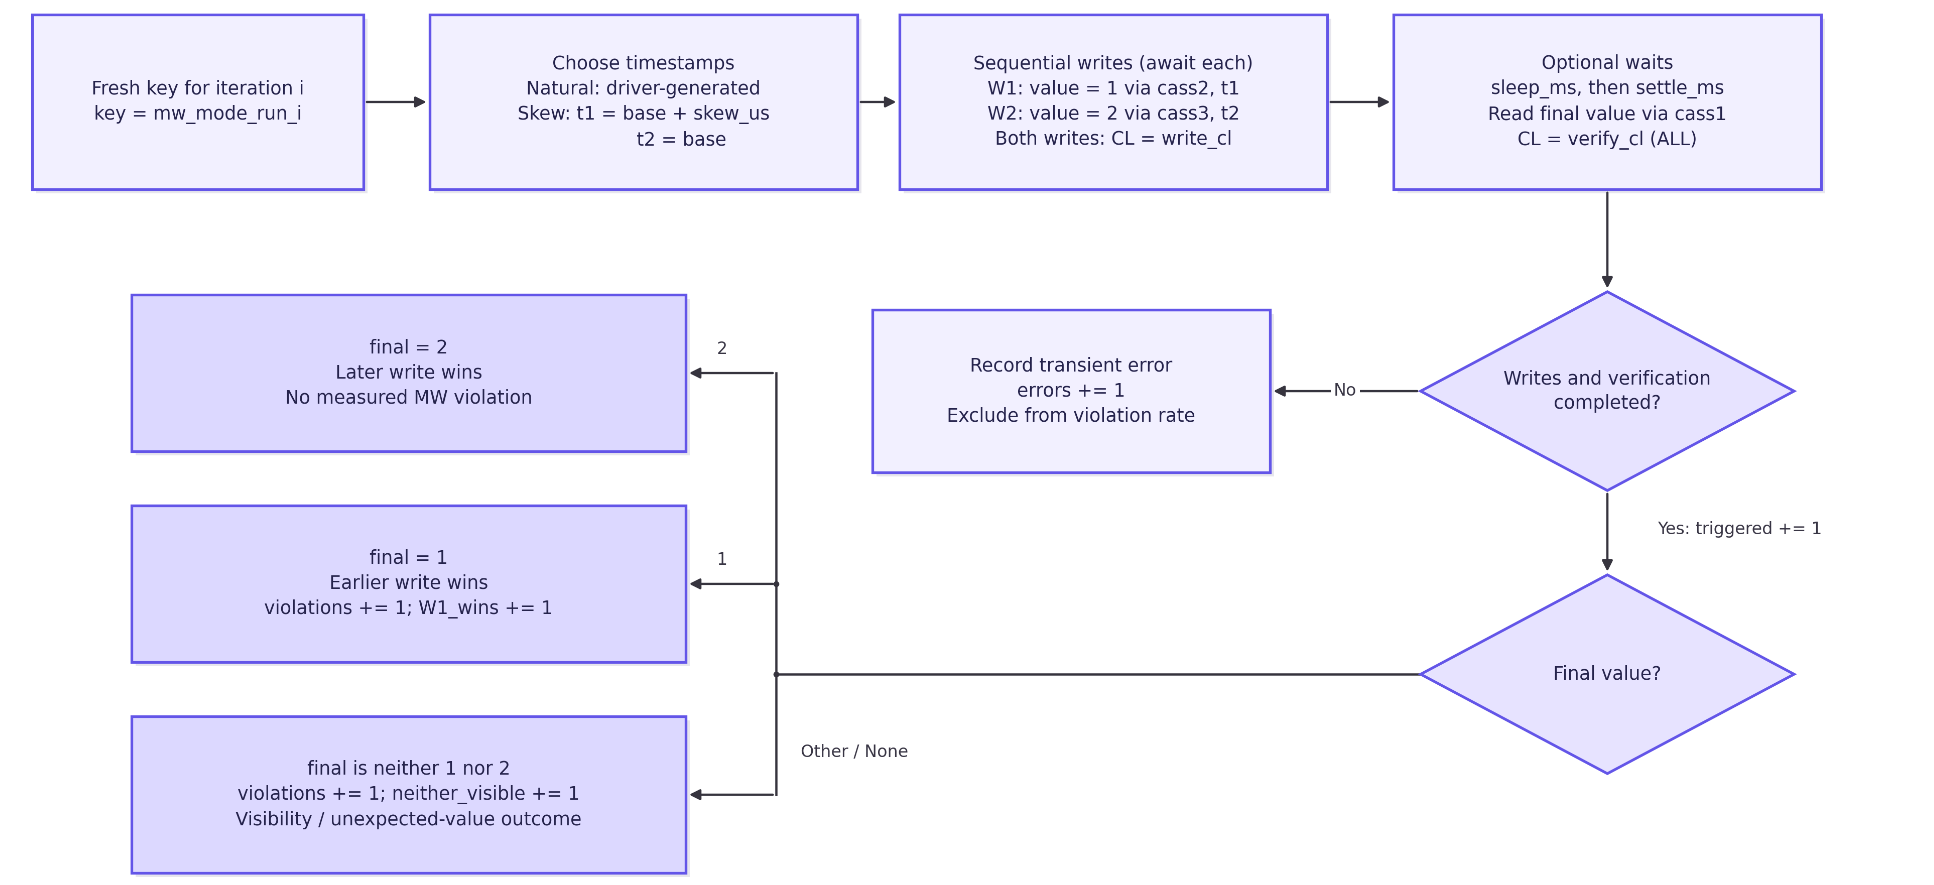
\includegraphics[width=\linewidth]{figures/mw_flow.png}
\caption{Monotonic-writes experimental workflow.}
\label{fig:mw-flow}
\end{figure}

The explicit-timestamp path uses INSERT \ldots{} USING TIMESTAMP. Verification uses SELECT value, writer, WRITETIME(value) \ldots. An ALL read reconciles responses from all replicas and reduces the risk of classifying a read from an uninformed replica as a write-order failure. It does not, by itself, prove that every replica has physically converged or reveal the order in which each replica applied mutations.

Although the matrix and plot retain read\_cl labels, the MW script does not use that parameter for verification. In the normal sweep every verification read uses ALL. Consequently, ONE--ONE and ONE--QUORUM are repeated tests with the same effective write and verification levels.

The driver documentation specifies a default monotonic timestamp generator per Cluster instance. Here, common.py creates a separate Cluster for each pinned node, so there is no explicitly shared generator across the two write connections. Increasing timestamps are expected under the observed sequential execution and stable client clock, but are not guaranteed across these separate generators merely by their individual monotonicity. \href{https://docs.datastax.com/en/developer/python-driver/3.29/api/cassandra/cluster/index.html}{DataStax Python driver documentation}.

\subsubsection{Predicted Outcomes}\label{mw:predicted-outcomes}

In natural mode, if W2 receives a greater timestamp than W1, value 2 should win reconciliation at every tested write consistency level. Delaying replication alone should not change that winner.

In skew mode, W1 has the greater timestamp by construction, despite W2 being issued later. Value 1 should therefore win, producing a 100\% measured violation rate under the script's final != 2 criterion. Raising write consistency to QUORUM or ALL cannot reverse the supplied timestamp order.

{
\begin{table}[H]
\centering
\small
\renewcommand{\arraystretch}{1.15}
\caption{Predicted MW outcomes under natural and inverted timestamp ordering.}\label{tab:mw-1}
\begin{tabular}{@{}
  >{\RaggedRight\arraybackslash}p{(\linewidth - 6\tabcolsep) * \real{0.2500}}
  >{\RaggedRight\arraybackslash}p{(\linewidth - 6\tabcolsep) * \real{0.2500}}
  >{\RaggedRight\arraybackslash}p{(\linewidth - 6\tabcolsep) * \real{0.2500}}
  >{\RaggedRight\arraybackslash}p{(\linewidth - 6\tabcolsep) * \real{0.2500}}@{}}
\toprule\noalign{}
\begin{minipage}[b]{\linewidth}\RaggedRight
Mode
\end{minipage} & \begin{minipage}[b]{\linewidth}\RaggedRight
Timestamp Relationship
\end{minipage} & \begin{minipage}[b]{\linewidth}\RaggedRight
Expected Winning Value
\end{minipage} & \begin{minipage}[b]{\linewidth}\RaggedRight
Expected Measured Rate
\end{minipage} \\
\midrule\noalign{}
natural & normally t2 \textgreater{} t1 & 2 & 0\% \\
skew & t1 = t2 + 500000 \(\mu\)s & 1 & 100\% \\
\bottomrule
\end{tabular}
\end{table}
}

\subsubsection{Results and Analysis}\label{mw:actual-results-and-analysis}

Across all ten delay settings, each retained mode/configuration row contains 100 valid iterations and zero operation errors.

{
\begin{table}[H]
\centering
\small
\renewcommand{\arraystretch}{1.15}
\caption{MW delay-sweep outcomes among successful verification reads.}\label{tab:mw-2}
\begin{tabular}{@{}llll@{}}
\toprule\noalign{}
W-R & Actual Verification CL & Natural Mode & Skew Mode \\
\midrule\noalign{}
ONE-ONE & ALL & 0\% at every delay & 100\% at every delay \\
ONE-QUORUM & ALL & 0\% at every delay & 100\% at every delay \\
QUORUM-QUORUM & ALL & 0\% at every delay & 100\% at every delay \\
ALL-ONE & ALL & 0\% at every delay & 100\% at every delay \\
\bottomrule
\end{tabular}
\end{table}
}

Detailed records can be found in \href{https://github.com/LuweiChenbot/Cassandra-Lab/blob/main/results/mw_windows.csv}{monotonic-write-records}. The two modes separate propagation delay from timestamp ordering. In natural mode, delayed delivery does not prevent the later write from winning reconciliation. In skew mode, the earlier write consistently wins because its assigned timestamp is larger. The result remains unchanged even when all replicas acknowledge both writes: stronger acknowledgements do not repair an inversion between application order and timestamp order.

The 500 ms skew is a difference between two assigned timestamps, not a waiting period. Therefore, increasing network delay beyond 500 ms does not remove the inversion; t1 remains greater than t2 regardless of elapsed execution time.

The main interpretive limitation is the measurement itself. The script tests whether the later application overwrite wins a reconciled read. It does not instrument per-replica mutation histories, enforce cross-key dependencies, or establish the full formal monotonic-writes property. The most precise conclusion is that natural execution preserved the intended overwrite result in all tested trials, while explicit timestamp inversion defeated that result at every tested write consistency level. The reported MW violation rate should be accompanied by this operational definition.

These findings indicate that preserving application write order requires attention to timestamp generation across the logical client session, including multiple connections or client instances. Raising consistency levels addresses acknowledgement and visibility requirements, but is insufficient to make timestamp-based conflict resolution follow application order when the timestamps themselves are inverted.

\paragraph{Detailed MW Results Across Topologies}\label{mw:detailed-mw-results-across-topologies}

The table below applies separately to both recorded partition/network settings, 0/0 ms and 100/50 ms. Normal has complete matrices at these settings as well as the ten-point zero-jitter sweep. Each natural or skew entry represents 100 attempted iterations per setting and row.

{
\begin{table}[H]
\centering
\small
\renewcommand{\arraystretch}{1.15}
\caption{MW results across topologies, applied separately at 0/0 ms and 100/50 ms delay/jitter.}\label{tab:mw-3}
\begin{tabular}{@{}
  >{\RaggedRight\arraybackslash}p{(\linewidth - 10\tabcolsep) * \real{0.1667}}
  >{\RaggedRight\arraybackslash}p{(\linewidth - 10\tabcolsep) * \real{0.1667}}
  >{\RaggedRight\arraybackslash}p{(\linewidth - 10\tabcolsep) * \real{0.1667}}
  >{\RaggedRight\arraybackslash}p{(\linewidth - 10\tabcolsep) * \real{0.1667}}
  >{\RaggedRight\arraybackslash}p{(\linewidth - 10\tabcolsep) * \real{0.1667}}
  >{\RaggedRight\arraybackslash}p{(\linewidth - 10\tabcolsep) * \real{0.1667}}@{}}
\toprule\noalign{}
\begin{minipage}[b]{\linewidth}\RaggedRight
Topology
\end{minipage} & \begin{minipage}[b]{\linewidth}\RaggedRight
W-R
\end{minipage} & \begin{minipage}[b]{\linewidth}\RaggedRight
Actual verification CL
\end{minipage} & \begin{minipage}[b]{\linewidth}\RaggedRight
Natural: violations/valid
\end{minipage} & \begin{minipage}[b]{\linewidth}\RaggedRight
Skew: violations/valid
\end{minipage} & \begin{minipage}[b]{\linewidth}\RaggedRight
Iteration error rate
\end{minipage} \\
\midrule\noalign{}
normal & ONE-ONE & ALL & 0/100 & 100/100 & 0\% \\
normal & ONE-QUORUM & ALL & 0/100 & 100/100 & 0\% \\
normal & QUORUM-QUORUM & ALL & 0/100 & 100/100 & 0\% \\
normal & ALL-ONE & ALL & 0/100 & 100/100 & 0\% \\
partition majority & ONE-ONE & QUORUM & 0/100 & 100/100 & 0\% \\
partition majority & ONE-QUORUM & QUORUM & 0/100 & 100/100 & 0\% \\
partition majority & QUORUM-QUORUM & QUORUM & 0/100 & 100/100 & 0\% \\
partition majority & ALL-ONE & QUORUM & N/A & N/A & 100\% \\
partition minority & ONE-ONE & ONE & 0/100 & 100/100 & 0\% \\
partition minority & ONE-QUORUM & ONE & 0/100 & 100/100 & 0\% \\
partition minority & QUORUM-QUORUM & ONE & N/A & N/A & 100\% \\
partition minority & ALL-ONE & ONE & N/A & N/A & 100\% \\
\bottomrule
\end{tabular}
\end{table}
}

Normal topology: delay changes delivery, while the assigned timestamps determine the observed winner. All writes and ALL verification reads complete at every supplied normal setting. Natural mode always returns the intended later value. Skew mode always preserves W1. The 100/50 ms jittered matrix agrees with the deterministic sweep. Thus neither zero jitter nor fixed packet timing is necessary for the observed timestamp-inversion outcome. These files contain outcome counts, not request-latency distributions, so they cannot quantify the performance cost of stronger CLs or larger delays.

Majority partition: verification is scoped to the two reachable replicas. W1 is sent through node 1 and W2 through node 2, with verification through node 1 at QUORUM. Both writes at ONE or QUORUM can finish within this component. The verification quorum covers both reachable replicas, and the matrix adds a settling interval. Natural mode returns 2; skew mode returns 1 at both 0/0 and 100/50 ms. ALL writes cannot obtain three acknowledgements, leaving no valid order check. Successful majority verification does not show that isolated node 3 has converged; it reports the reconciled outcome available within the majority.

Minority partition: timestamp inversion occurs even without changing nodes. W1, W2, and verification all use node 3. With W=ONE, natural mode returns 2, but skew mode still returns 1 in every trial. This is particularly informative: the undesired overwrite result can arise entirely on one replica when the application supplies inverted timestamps. Neither cross-node delivery reordering nor communication with another replica is necessary to produce it. Network partitioning determines which CLs remain usable, while the explicit timestamp order determines which of the two values wins locally.

The nominal ONE--QUORUM minority row completes because the MW script never executes a read at its read\_cl label: it uses verify\_cl=ONE. This explains the apparent contrast with MR, where ONE--QUORUM fails on the minority because an actual quorum read is attempted. Comparing the two models solely by plot legends would therefore give a misleading availability conclusion.

Unavailable configurations. Both modes fail at ALL on the majority and at QUORUM or ALL on the minority. A zero stored violation count in these rows means no successful verification was available, not that timestamp skew was harmless. The correct outcome is ``ordering result unavailable; iteration error rate 100\%.''

\paragraph{Full-Dataset Accounting and Scope of the MW Claim}\label{mw:full-dataset-accounting-and-scope-of-the-mw-claim}

The following totals retain every supplied row, including repeated zero-delay normal baselines. They are an inventory of evidence, not a balanced estimate across operating conditions.

{
\begin{table}[H]
\centering
\small
\renewcommand{\arraystretch}{1.15}
\caption{Full-dataset MW accounting by topology and timestamp mode.}\label{tab:mw-4}
\begin{tabular}{@{}
  >{\RaggedRight\arraybackslash}p{(\linewidth - 8\tabcolsep) * \real{0.2000}}
  >{\RaggedRight\arraybackslash}p{(\linewidth - 8\tabcolsep) * \real{0.2000}}
  >{\RaggedRight\arraybackslash}p{(\linewidth - 8\tabcolsep) * \real{0.2000}}
  >{\RaggedRight\arraybackslash}p{(\linewidth - 8\tabcolsep) * \real{0.2000}}
  >{\RaggedRight\arraybackslash}p{(\linewidth - 8\tabcolsep) * \real{0.2000}}@{}}
\toprule\noalign{}
\begin{minipage}[b]{\linewidth}\RaggedRight
Topology
\end{minipage} & \begin{minipage}[b]{\linewidth}\RaggedRight
Mode
\end{minipage} & \begin{minipage}[b]{\linewidth}\RaggedRight
Attempted iterations
\end{minipage} & \begin{minipage}[b]{\linewidth}\RaggedRight
Valid iterations
\end{minipage} & \begin{minipage}[b]{\linewidth}\RaggedRight
Measured violations
\end{minipage} \\
\midrule\noalign{}
normal & natural & 4800 & 4800 & 0 \\
normal & skew & 4800 & 4800 & 4800 \\
partition majority & natural & 800 & 600 & 0 \\
partition majority & skew & 800 & 600 & 600 \\
partition minority & natural & 800 & 400 & 0 \\
partition minority & skew & 800 & 400 & 400 \\
\bottomrule
\end{tabular}
\end{table}
}

Across all settings, natural mode has 0/5,800 measured violations among valid iterations, while skew mode has 5,800/5,800. Each mode also has 600 unavailable iterations. The 4,000-trial figures reported for the sweep refer only to its retained ten-delay subset and should not be confused with these whole-file totals.

The decisive comparison is conditional on successful verification: natural and skew modes yield opposite winners under every available tested configuration. The minority experiment shows that timestamp inversion is sufficient even locally; the normal ALL-write experiment shows that acknowledging every replica does not correct it. Together, these results substantiate a failure to preserve the application's intended overwrite order under inverted timestamps. They do not directly observe every replica's mutation order or establish a complete formal test of monotonic writes across multiple keys.

The full dataset consequently distinguishes three experimentally different effects: replication timing influences the opportunity for backwards reads; network reachability determines whether selected CLs can complete; and supplied timestamp order controls the winning overwrite in the MW test. Keeping these dimensions separate explains the observed curves, the majority/minority asymmetry, and the apparently conflicting zero and 100\% results.
